\documentclass[12pt, a4paper, oneside]{book}
 
% - taille de la fonte    : 10pt, 11pt, 12pt
% - recto ou recto-verso    : oneside, twoside
 
% Chargement d'extensions
\usepackage[utf8]{inputenc}
\usepackage[T1]{fontenc}
\usepackage[francais]{babel}
\usepackage[margin=1in]{geometry}
\usepackage{url}
\usepackage{graphicx}
\usepackage{caption}
\usepackage{subcaption}
\usepackage{eurosym}
\usepackage{float}
\usepackage{csquotes}

\DeclareUnicodeCharacter{202F}{FIX ME!!!!}

% Informations le titre, le(s) auteur(s), la date
\title{La Blockchain}
\author{ Jordan Sagnes, Alexandre Ludwig, Yoan Fath, \\ Julien Pignolet et Arnaud Couderc}
\date{\today}

 
\begin{document}
\maketitle
 
    % Le prologue du livre
    \frontmatter
    
    %\section{Introduction}
    
    \tableofcontents
    \thispagestyle{empty}
    % Corps du livre
    \mainmatter

    \chapter{Introduction à la blockchain}
    \section{Nouvelle technologie - Historique}
    En 1991 l’architecture de la blockchain a été décrite par les chercheurs Stuart Haber et W. Scott Stornetta lors d’une recherche permettant l’horodatage de documents numériques assurant qu’ils ne soient jamais antidatés ou altérés. 
	Ils ont créé une entreprise de certification et ont commencé à utiliser le principe de la blockchain en publiant une attestation cryptographique de la base de données des sceaux numérique dans la section « Annonces et objets trouvés » du New York Times. Cette attestation était une chaine de caractère des empreintes de tous les fichiers encodés en base64. A l’époque il y avait 600 000 tirages par jour, ce qui fait que pour altérer des données il aurait fallu récupérer tous ces exemplaires et les remplacer par une version falsifiée.  
	En 1992, le protocole \hyphenquote{french}{ arbre de Merkle } fut utilisé pour combiner plusieurs documents dans un seul bloc. 


En 2008, la publication d’un livre blanc par un inconnu se présentant sous le pseudonyme Satoshi Nakamoto, signe le retour de la blockchain. Son but était d’introduire un système de paiement électronique décentralisé peer-to-peer, le Bitcoin.
    \section{Qu'est-ce que la blockchain ?}
    La blockchain est une architecture de stockage de données et de transmissions d’informations sécurisées qui fonctionnent de manière décentralisée, avec des blocs de données reliés entre eux. Elle contient l’historique de toutes les transactions effectuées entre les utilisateurs depuis sa création. 

La blockchain est un système fondé sur le principe de preuves. Elles nécessitent une puissance de calcul importante, fournie par les mineurs, notamment pour ouvrir un nouveau bloc pour y inscrire les données et pour vérifier la validité d’un bloc. Le détail du fonctionnement sera expliqué dans la partie technique.

\begin{figure}[H]
    \begin{center}
      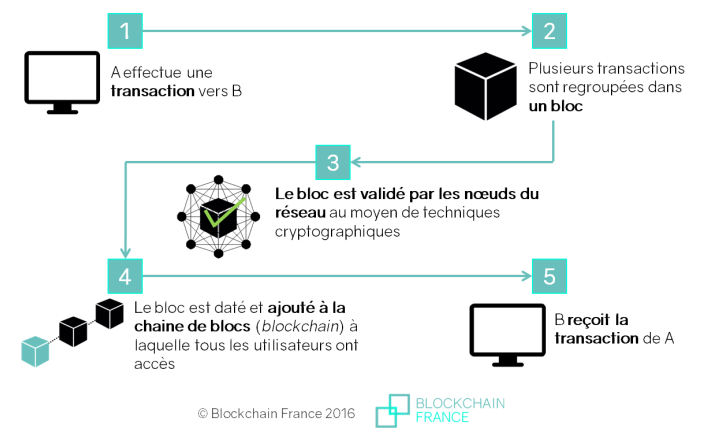
\includegraphics[width=.55\textwidth]{images/blockchain.png}
      \label{fig:blockchain}
      \caption{La blockchain}
    \end{center}
\end{figure}

Tous les échanges dans la blockchain sont anonymes, consultables, et non modifiables. Il n'y a besoin d'aucun tiers de confiance, l’ensemble du réseau se chargeant d’authentifier les transactions avec la méthode de cryptographie utilisée.

\section{La décentralisation des données}
    Le fait que la blockchain soit décentralisée et partagée entre ses utilisateurs permet la vérification de l’intégrité de la chaine par n’importe quel utilisateur, même les créateurs n’ont aucun pouvoir unilatéral sur la blockchain (censure) ou la modification du fonctionnement, ce qui est totalement différent des applications proposées par exemple, par les GAFAM.

Avec la décentralisation des données, l’utilisateur est maître de ses données personnelles et de son identité numérique, il peut choisir les services qui accèderont à ses données et en monnayer l’accès, tout en pouvant révoquer ce dernier lorsqu'il le souhaite. Cela permet de présenter une facette de son identité en fonction du contexte. 

\section{Les tokens}
Toute blockchain publique fonctionne obligatoirement avec un jeton : \hyphenquote{french}{ le Token }. Il est programmable et personnalisable pour représenter ce qui sera échangé. Cela peut être une cryptomonnaie, un droit d’usage, un droit de paiement, une réputation… Cela peut prendre n’importe quelle forme et c’est ce qui sera utilisé et échangé en peer-to-peer sans duplication sur la blockchain.
Ce token peut être acheté et vendu n’importe quand en fonction de l’offre et de la demande sur une plateforme d’échange, son prix n’est jamais fixe mais varie tout le temps. 

Un token conserve toutes les caractéristiques d’une cryptomonnaie : infalsifiable, enregistrement de la transaction dans un bloc immuable, sécurité des échanges.

\section{Le Bitcoin et les cryptomonnaies dans tout ça ?}
La première blockchain qui s’est développée en 2009 est un système de paiement qui utilise une cryptomonnaie comme token : le bitcoin. 
A chaque transaction réalisée, les agents qui traitent et vérifient les transactions sont rétribués, ce sont les mineurs. Le fait de miner consiste à vérifier, sécuriser et enregistrer une transaction et des bitcoins sont générés dans le système, à chaque nouveau bloc créé.
 Le système à une limite de 21 millions d’unités sur le marché et, d’après les estimations, ce cap sera atteint d’ici 2050, ceci rendra le bitcoin encore plus rare car limité. Le bitcoin, comme toute cryptomonnaie peut être échangé sur des places de marchés avec la loi de l’offre et de la demande, ce qui peut grandement faire varier le prix comme en 2017 lorsque le prix du bitcoin a explosé dû à la demande.

Le bitcoin prend une place importante sur le marché car il s'est fait connaitre d'un coup et son intérêt a engendré de nombreux achats en une petite période de temps. En outre, la blockchain sécurise les transactions et la faillite ou les scandales bancaires comme la Lehman Brothers~\cite{Lehman} ont fait vasciller la confiance du peuple envers ces établissements.
De plus le nombre de commerçants qui acceptent les bitcoins augmentent petit à petit, comme Microsoft ou Steam pendant un temps, ce qui rend l'utilisation des bitcoins moins compliquée.

\section{Les 3 types de blockchain}

Il existe 3 types de blockchain :
\\

\begin{itemize}


\item Publique : tout le monde peut lire, envoyer et participer à l'approbation des transactions dans le registre.\\

\item Privée : Les permissions d'accès, de lecture et de vérification du registre de la Blockchain peuvent être contrôlés pour limiter les accès tout en conservant les avantages de la technologie comme l'authenticité, ou la décentralisation.\\

\item Consortium : Dans un consortium le processus d'approbation peut être contrôlé par un nombre défini de nœuds. Par exemple, une dizaine d'institutions peuvent se mettre d'accord pour dire qu'il faut au moins que 8 d'entre elles approuvent le bloc avant qu'il soit considéré comme valide. Cela modifie donc le comportement original car ce n'est plus la règle de majorité qui compte mais ce sont les participants au processus d'approbation qui ont été sélectionnés qui vont décider.\\

\end{itemize}
 
    
    \chapter{Les applications de la blockchain}

    Majoritairement, lorsqu’on parle de blockchain, le premier mot qui nous vient à l’esprit est bitcoin. Peut-être à juste titre, car les cryptomonnaies représentent l’application la plus médiatisée de la blockchain. Mais saviez-vous que le domaine de la Finance n’est pas le seul à être courtisé par la blockchain ? Nous avons choisi de vous parler d’applications plus à la marge, qui pourraient révolutionner leurs domaines.

    \section{L'industrie du jeu video}

    Il y a une large variété d’implémentation possible de la blockchain dans le domaine du jeu vidéo~\cite{JV}, au-delà de l’utilisation de cryptomonnaies pour les microtransactions.  L’aspect infalsifiable du registre de transaction pourrait permettre aux jeux vidéo de se prémunir de la triche.
    \\
    C’est dans la gestion de la progression du joueur que la blockchain pourrait intervenir. En effet, la valeur d’un joueur est souvent associée à la quantité de pièces et d’objets brillants qu’il a pu acquérir en complétant des niveaux, succès, etc... La progression représente la colonne vertébrale de la plupart des jeux et sécuriser celle-ci, en la rendant infalsifiable, semble donc essentiel.
    \\
    Un exemple concret de l'importance de la sécurisation de ces données est Miniclip’s 8-Ball Pool. Il s’agit d’un jeu mobile de billard, où quelques joueurs ont réussi acquérir des avantages beaucoup plus tôt que prévu dans le jeu, leur donnant ainsi un avantage déloyal face aux joueurs honnêtes décourageant ces derniers de jouer.
    
    \begin{figure}[H]
        \begin{center}
          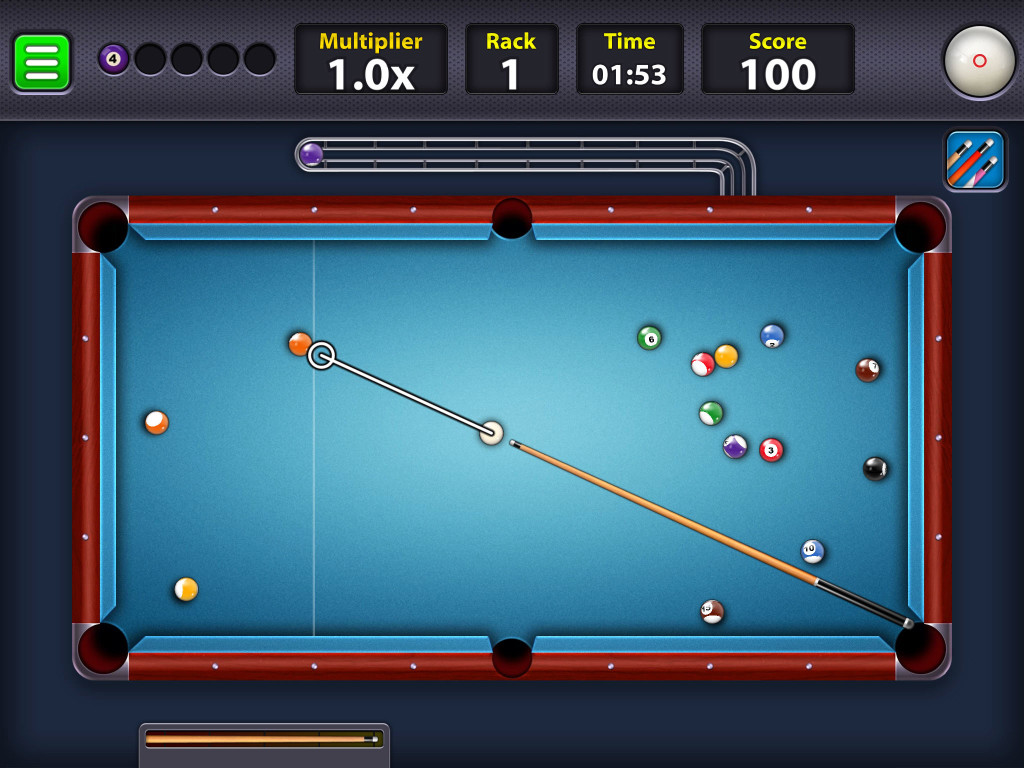
\includegraphics[width=.43\textwidth]{images/billard.jpg}
          \label{fig:billard}
          \caption{Miniclip’s 8-Ball Pool : Un jeu mobile qui pourrait utiliser la blockchain}
        \end{center}
    \end{figure}
    Ainsi, des jeux comme Gods Unchained, basés sur la blockchain, ont commencés à voir le jour. Il s'agit d'un jeu de cartes, qui, pour les connaisseurs ressemble énormément à Hearthstone. A un détail près, les cartes sont limitées et identifiées de manière unique à l'aide d'un token. Chaque carte vaut d'ailleurs une certaine somme en Ethereum. Petite anecdote, un concours pour remporter une carte dont la valeur est estimée à 60 000 \euro~est en cours. Tout l'intérêt de la blockchain, est l'identification unique des cartes (et l'aspect infalsifiable du registre) empêchant un pirate d'introduire des cartes illégitimes dans le jeu.
    
    \begin{figure}[H]
        \begin{center}
          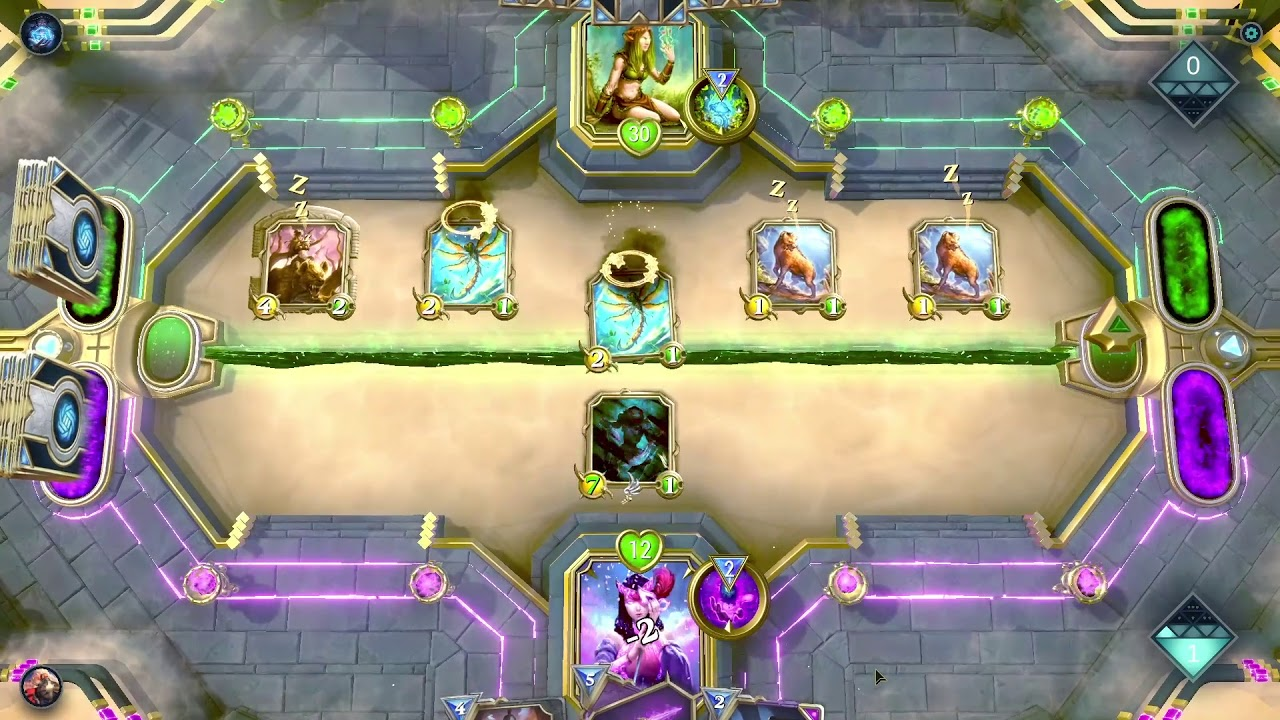
\includegraphics[width=.69\textwidth]{images/godsunchained.jpg}
          \label{fig:jeucartes}
          \caption{Gods Unchained : un jeu utilisant la blockchain}
        \end{center}
    \end{figure}

    Il semblerait que le géant Ubisoft~\cite{ubi} soit en train de mettre en place ce genre de solution.

    \section{L'industrie agroalimentaire}

    En parlant de géants, dans un tout autre domaine cette fois, Carrefour et Nestlé ont eux aussi adoptés la blockchain en s’alliant à IBM et sa solution IBM Food Trust~\cite{IBMfood}.
    \\
    Le postulat de base est simple : Les consommateurs n’ont jamais eu autant de choix dans la diversité de leurs aliments. Pourtant d’après IBM, 84\% des acheteurs considèrent au moment de leur achat, où et comment ont été produits les aliments. C’est là que la blockchain peut être décisive. Dans un milieu aussi compétitif, elle permet une transparence totale de la chaîne d’approvisionnement et de fabrication, toujours grâce à l’aspect infalsifiable du registre de transaction.
    \\
    D’après Nestlé, cela permet de \hyphenquote{french}{ renforcer le lien de confiance avec ses consommateurs }. C’est pourquoi ces derniers appliquent cette solution sur 15 de leurs produits phares, notamment la purée Mousline. Carrefour compte quant à lui déployer cette solution d’ici 2020 sur l’ensemble des produits alimentaires Filière Qualité Carrefour, soit 300 références.
    \\
    Assurer la traçabilité des produits représente aussi un avantage majeur en cas d’incident de sécurité alimentaire. Certaines compagnies, prennent parfois plusieurs jours à plusieurs semaines pour retracer leur propre chaine.
    \\
    En généralisant, la plus grosse vulnérabilité de la chaîne d’approvisionnement est le manque de transparence car c'est une porte ouverte vers la fraude et la corruption (exemple de la fraude sur l’étiquetage faisant passer de la viande de cheval pour de la viande de bœuf), problème qui est résolu par la blockchain.

    \section{Les Smart Contracts}
    Les smart contracts constituent l’un des types d’usage les plus prometteurs de la blockchain. Concrètement, il s’agit d’un programme informatique qui exécute automatiquement des conditions définies au préalable et inscrites dans la blockchain. Un smart contract est beaucoup plus simple qu’il n’y paraît. Il fonctionne comme toute instruction \hyphenquote{french}{ if – then }. 
    \\
    \indent
    Pour illustrer, saviez-vous que 60\% des passagers assurés contre le retard de leur vol ne revendiquaient jamais leur argent ? C’est à partir de ce constat qu’un système d’assurance automatisé basé sur les smart contracts est né. AXA est l’un des premiers grands groupes d’assurance à l’adopter. Le principe ? Les passagers sont automatiquement indemnisés lorsque leur vol est en retard, sans avoir besoin de remplir un quelconque formulaire, et donc sans que l’entreprise ne doive traiter les demandes. Pour se déclencher, le smart contract se connecte à une base de données supposée fiable, dans le cas présent la base de données de l’aéroport.
    Le smart contract est indissociable de la blockchain car elle permet de se passer d’un tier de confiance pour les phases déclaratives.
    \\
    \indent~
    L’avantage des smarts contracts c’est, qu’une fois inscrits dans la blockchain, les termes du contrat ne pourront plus être modifiés. On retrouve encore une fois l’aspect indissociable de la blockchain. Car un smart contract qui ne serait pas dans la blockchain serait un programme dont les termes pourraient être changés en cours d’exécution.
    Les smarts contracts permettent aussi de réduire les coûts de vérification, d’exécution, d’arbitrage et de fraude. Tout est automatisé donc plus aucune erreur humaine n’est possible, sauf au moment d’établir le contrat.


    \chapter{Blockchain dans sa technique}
    \section{Introduction}
    Nous allons illustrer le fonctionnement de la blockchain avec un exemple : Alice, Bob et Eve qui souhaitent mettre en place une méthode sécurisée pour gérer leur argent ainsi que leurs transactions.

    \section{Qu'est-ce que la blockchain ?}
    Imaginons un livre dans lequel nous pouvons tout noter. Dans notre exemple, Alice pourra alors y indiquer le montant disponible sur son compte et toutes ses transactions réalisées. Une fois qu’une page est remplie, nous passons simplement à la page suivante.
    \\
    La blockchain fonctionne sur ce même principe sauf qu’en réalité les pages sont appelées des blocs, et une fois que le nombre de transaction maximal est atteint, nous ouvrons un nouveau bloc.

    \section{Fonctionnement de la blockchain}
    
    \subsection{Disponibilité de la blockchain}
    La blockchain est un réseau décentralisé qui fonctionne sur le principe du Peer-to-peer (P2P). 
    Ainsi un serveur principal partage avec tout le réseau les nouvelles modifications, mais là où est la force d'un réseau pair à pair, c'est que les clients se partagent aussi 
    entre eux les informations qu'ils connaissent déjà. De ce fait, les données sont alors disponibles en permanence. Le seul moyen de les rendre inaccessibles serait une 
    coupure internet mondiale, or pour lutter contre ce problème certaines blockchains prévoient d'utiliser des satellites.
    
    \begin{figure}[H]
        \begin{center}
          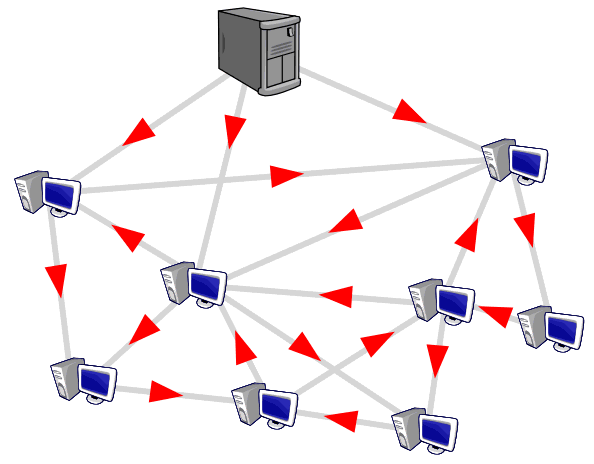
\includegraphics[width=.69\textwidth]{images/peerToPeer.png}
          \label{fig:peerToPeer}
          \caption{Blockchain : Un réseau Peer-to-peer}
        \end{center}
    \end{figure}

    \subsection{Intégrité d'un bloc}
    Il est important que toutes les données stockées dans la blockchain soient intègres, c’est-à-dire qu’il faut être sûr qu’elles n’aient pas été modifiées maladroitement ou par un utilisateur mal intentionné.
    \\
    Mettons en place notre exemple :

    \begin{enumerate}
        \item Alice, Bob et Eve possèdent tous 10 \euro~sur leur compte et n’ont encore effectué aucune transaction.
        \item Il n'y a aucune mesure de sécurité en place, Eve décide de modifier les données et de voler de l’argent à Alice. 
        \newline
    \end{enumerate} 

    \begin{figure}[H]
        \centering
        \begin{subfigure}{.5\textwidth}
          \centering
          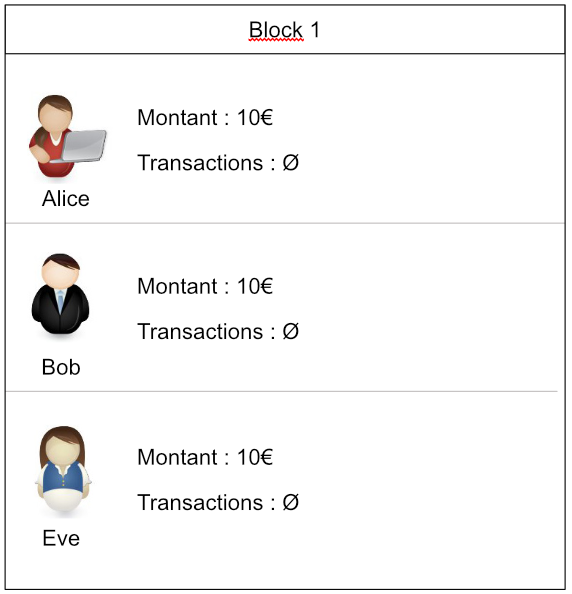
\includegraphics[width=.7\textwidth]{images/bloc1.png}
          \label{fig:bloc1}
        \end{subfigure}%
        \begin{subfigure}{.5\textwidth}
          \centering
          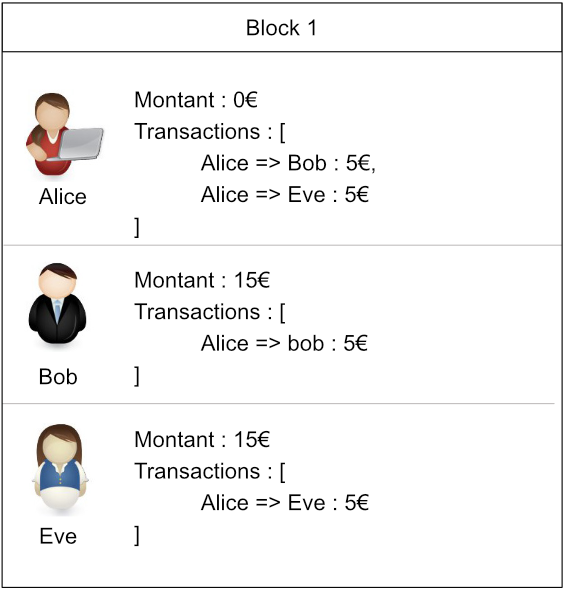
\includegraphics[width=.7\textwidth]{images/bloc2.png}
          \label{fig:bloc2}
        \end{subfigure}
        \caption{Le livre est ouvert, n'importe qui peut faire n'importe quoi.}
        \label{fig:test}
    \end{figure}

    Pour remédier à ce problème, une première solution est de hacher le contenu d’un bloc et d’inscrire le résultat dans celui-ci, or un hachage est très rapide à réaliser et donc rien ne pourrait empêcher Eve de modifier les données puis recalculer un nouveau hash.

    \begin{figure}[H]
        \begin{center}
          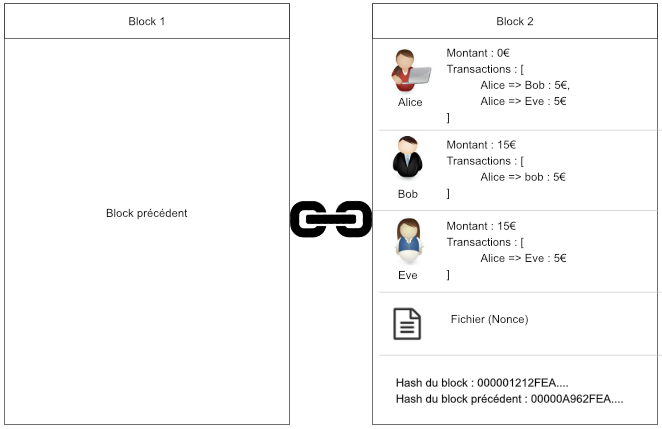
\includegraphics[width=.98\textwidth]{images/chaine.png}
          \label{fig:chaine}
          \caption{Une chaine de bloc : un bloc est lié à son prédecesseur par le hash de ce dernier.}
        \end{center}
    \end{figure}
    Une modification des informations présentes dans un bloc est donc nécessaire :
    \\
    \begin{itemize}
        \item En plus des informations déjà présentes, nous avons maintenant le hash du bloc précédent et le hash du bloc actuel : Pour l’obtenir nous hachons la totalité des informations, les transactions, le fichier nonce et le hash du bloc précédent.
        \item Un nonce est un fichier généré aléatoirement pour que le hash du bloc suive une règle précise (ici commencer par cinq zéros consécutifs). Nous reviendrons plus précisément sur ce sujet dans la partie Proof Of Work.
    \end{itemize}


    Maintenant, si Eve tente de modifier les données d’un bloc, il faudra qu’elle régénère le fichier nonce pour que le hash suive toujours la règle imposée, or cette opération est impossible à réaliser pour une seule personne car le nombre d’opérations à effectuer est très élevé. De plus si jamais Eve arrive par chance à en trouver un nouveau il faut qu’elle recommence pour tous les blocs suivants car elle aura modifié le hash du bloc précédent.

    \subsection{Intégrité du contenu d’un bloc}

    Dans la partie précédente nous avons vu comment nous assurer que les blocs sont intègres. Mais comment savoir avant d’ajouter des transactions dans un bloc que celles-ci n’ont pas été modifiées ?
    
    Pour cela nous allons utiliser un arbre de Merkle, inventé en 1979 par Ralph Merkle. Il s’agit d’un arbre de hachage binaire, son but est donc de vérifier l’intégrité d’un groupe de données (ici des transactions) sans devoir nécessairement utiliser toutes les données disponibles dans un bloc.

    \begin{figure}[H]
        \begin{center}
          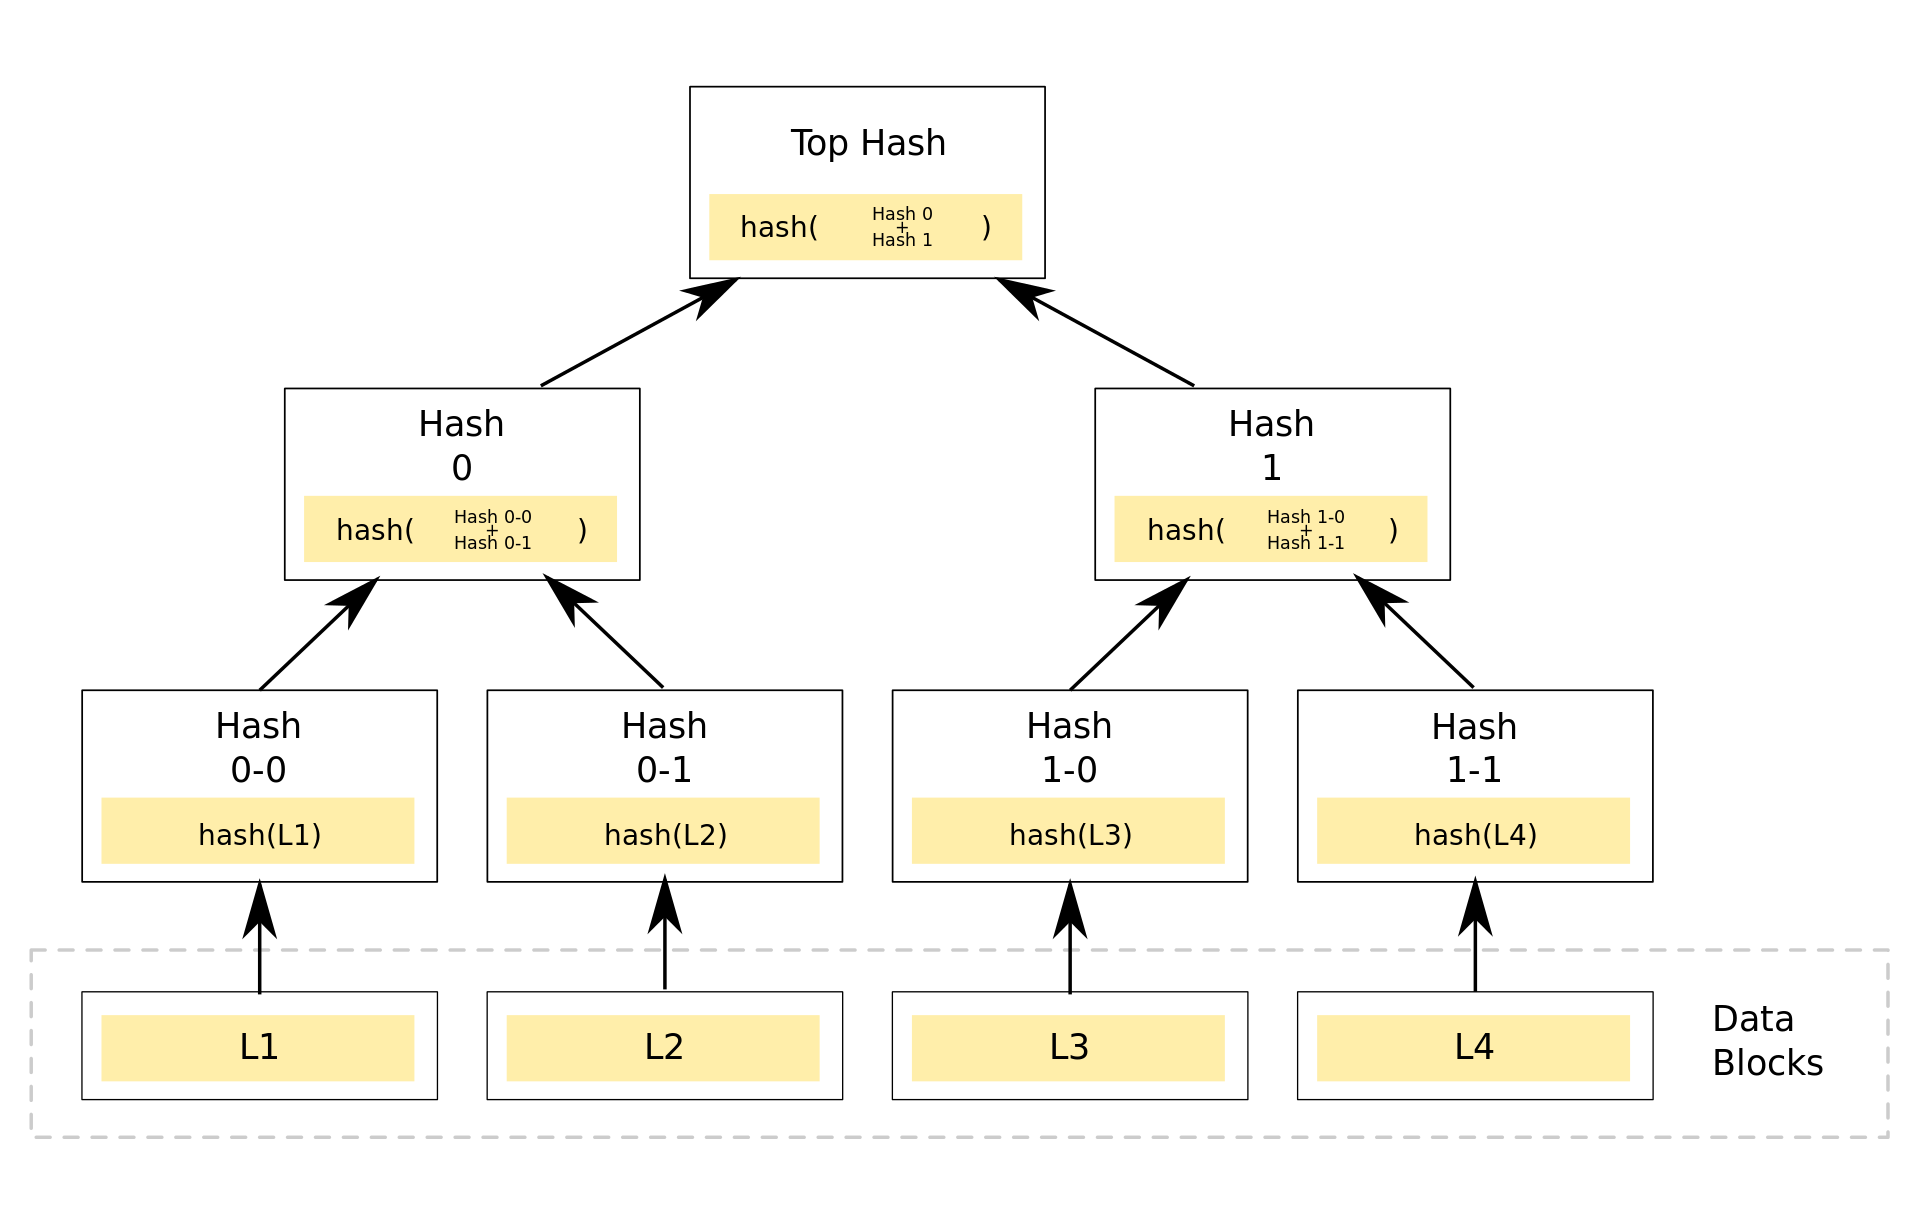
\includegraphics[width=\textwidth]{images/arbre.png}
          \label{fig:arbre}
          \caption{Un arbre de Merkle appliqué à la blockchain.}
        \end{center}
    \end{figure}
    \newpage
    \noindent~Sur le schéma ci-dessus et en considérant que nous sommes encore dans notre exemple :

    \begin{itemize}
        \item Les feuilles (Hash 0-0, Hash 0-1, …) représentent le hash des transactions
        \item Un parent représente le hash de ses deux enfants
        \newline
    \end{itemize}
    Si nous voulons vérifier l’intégrité de la transaction L3 (Hash 1-0), nous devons seulement posséder le hash de son frère (Hash 1-1), celui de son oncle (Hash 0) et enfin la racine (le Top Hash).
    
    Pour cette opération il suffit d'être sûr de l’intégrité du \hyphenquote{french}{ Top Hash }, c’est pourquoi cette information sera rajoutée au contenu d’un bloc dont l'intégrité a été prouvée dans le point précédent.\cite{merkle}
    
    \subsection {Confidentialité de la blockchain}
    La confidentialité correspond à la protection des données. En d’autres termes, si nous lions ça à la blockchain, cela signifie que la transaction et l’identité des participants doivent être protégés. 
    
    Reprenons notre exemple :
    Nos deux amis Alice et Bob possèdent 10 \euro~sur leur compte et Bob souhaite envoyer 5 \euro~à Alice. 
    
    Si nous voulons que leur transaction soit confidentielle, il faut que Eve soit incapable ni d’identifier que Alice et Bob se sont échangés de l’argent, ni le montant échangé. Sauf si Alice et Bob décident volontairement de révéler ces informations.
    
    Il faut savoir que dans la blockchain, toutes les transactions sont publiques. Ainsi Eve peut facilement avoir accès à la transaction, pour peu qu’elle ne soit pas encryptée. Ce qui est le cas de beaucoup de transactions publiques. 
    
    Voici un exemple de transaction tiré de blockchain.com : nous savons les adresses publiques des acteurs de la transaction, ainsi que la date et le montant de la transaction. Le montant que possède ces deux adresses dans leur portefeuille est aussi disponible.

    \begin{figure}[H]
        \begin{center}
          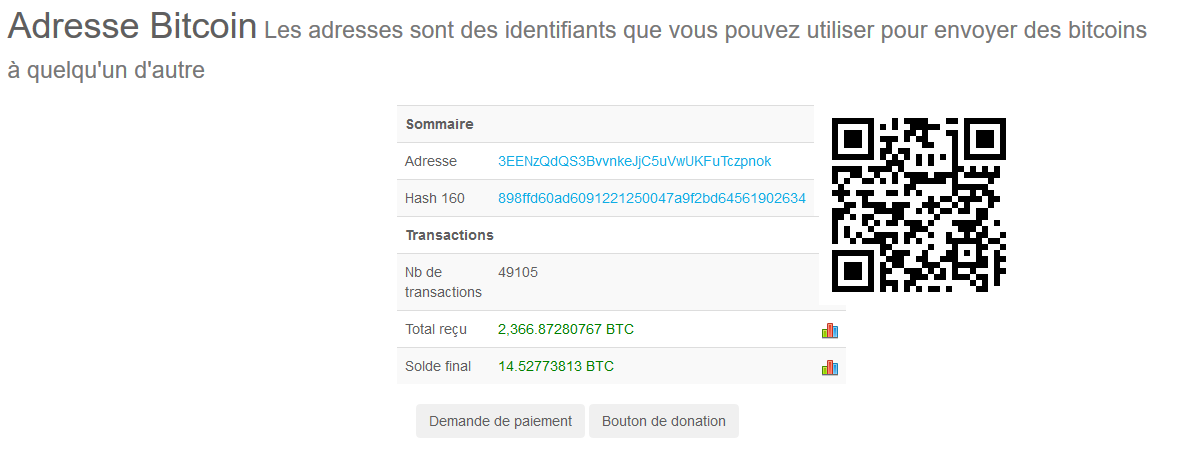
\includegraphics[width=\textwidth]{images/portefeuille.png}
          \label{fig:portefeuille}
          \caption{Un portefeuille Bitcoin}
        \end{center}
    \end{figure}

    \begin{figure}[H]
        \begin{center}
          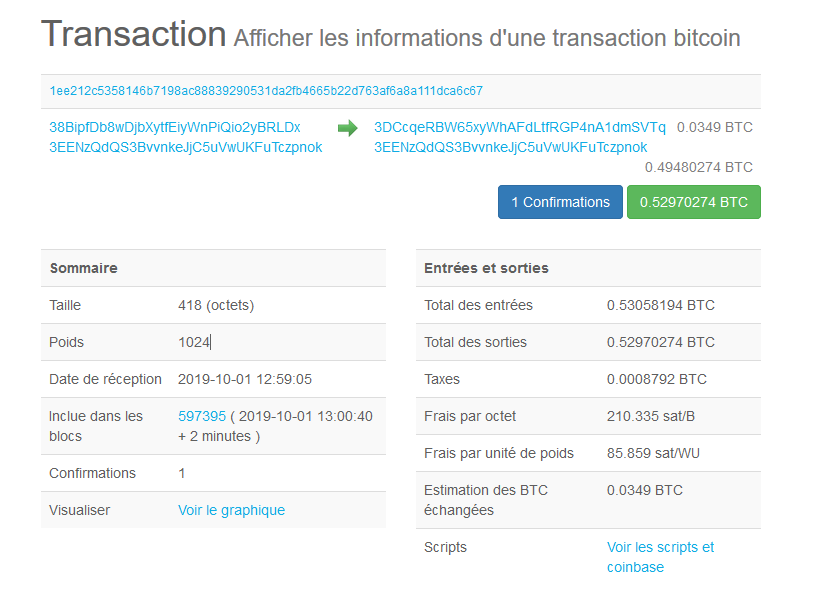
\includegraphics[width=.9\textwidth]{images/transaction.png}
          \label{fig:transaction}
          \caption{Une transaction Bitcoin}
        \end{center}
    \end{figure}

    Si l’on veut que la transaction soit confidentielle. Il faut donc que Bob encrypte les informations de celle-ci avec la clé publique de Alice, afin que seul Alice puisse décrypter la transaction avec sa clé privée. 
    
    Le problème du cryptage, c’est qu’il rompt l’un des principes fondamentaux de la blockchain, la transparence. C’est pourquoi, pour le moment, les transactions des blockchains publiques ne sont pas confidentielles. Comme nous avons d’ailleurs pu le voir sur l’image ci-dessus. Il s’agit d’ailleurs d’un sujet actif de recherche. 


    \subsection{Traçabilité}
    Comme nous l’avons vu dans les points précédents, la blockchain peut être vue comme un livre dans lequel nous écrivons absolument tout :
    \begin{itemize}
        \item Qui a effectué ce virement ?
        \item De quel montant est ce virement ?
        \item Qui a reçu le virement ?
        \newline
    \end{itemize}
    Le fait d'avoir la certitude que les informations soient intègres nous permet donc de valider que la blockchain respecte la notion de traçabilité. Ainsi, si nous revenons à notre cas d’application, nous pouvons par exemple avoir accès à tous les anciens propriétaires du dernier billet de 10~\euro~ reçu par Alice. Nous avons aussi vu l’exemple de Carrefour qui utilise la blockchain spécifiquement pour la traçabilité de ses produits.

    \subsection{Proof-of-Work}

    Le Proof of Work (PoW ou preuve de travail) est plus communément appelé minage. Les utilisateurs (Alice, Bob et Eve) disposent donc chacun d’une copie de la blockchain et ils ont différentes missions :

    \begin{itemize}
        \item Vérifier l’intégrité des blocs et des transactions : Ces opérations sont très rapides, il s’agit simplement de vérifier les hashs.
        \item Créer / ouvrir des nouveaux blocs : Comme nous l’avons vu précédemment cette opération consiste à trouver un fichier \hyphenquote{french}{ nonce } afin que le hash du bloc respecte certaines règles et donc sécuriser la blockchain. Cela prend énormément de temps de calcul et par conséquent provoque un réel impact écologique (électricité).
        \newline
    \end{itemize}

    Lorsqu’un mineur trouve un nonce correct il le diffuse sur le réseau, les autres mineurs vérifient ce fichier et selon sa validité, le mineur est alors récompensé, en effet il va percevoir tous les frais de transactions du bloc.
    \newline

    Chaque cryptomonnaie impose un délai avant de pouvoir ouvrir un nouveau bloc, par exemple pour le bitcoin, il y a environ un nouveau bloc toutes les 10 minutes.
    Plus il y aura de mineurs sur un réseau plus la difficulté augmentera, c'est-à-dire les règles sur l'aspect que doit avoir le hash seront de plus en plus complexes et donc le fichier nonce sera bien plus dur à trouver. \newline
    Or, le fait que la génération de nonce soit purement aléatoire fait que ce procédé peut poser problème. Par exemple le 30 septembre 2019 pour la dixième fois depuis 2004, un bloc a été miné en seulement 2 minutes (0.000679\% de chance),
    ainsi la difficulté a été grandement augmentée et par conséquent le prochain bloc a été miné en 2h ce qui a engendré des retards de paiements.

    \subsection{Proof-of-Stack}
    Ce principe remplace de plus en plus le Proof of Work car son concept est beaucoup moins énergivore. Le Proof Of Stack est comparable à un livret A : Nous sommes rémunérés un certain pourcentage pour garder des cryptomonnaies sur un serveur (cela s’appelle un masternode).
    Au lieu de générer un fichier aléatoire pour valider un bloc, un leader va être élu pour en créer un nouveau qu’il pourra signer. Pour éviter toute tentative de fraude, il devra auparavant miser une certaine somme définie qui lui sera restituée quand le bloc aura été validé par les autres membres du réseau.


    \chapter{Risques, vulnérabilités et attaques sur la blockchain}
    La blockchain n'est pas inviolable, mais comme souvent, les failles présentes sont dues à des erreurs d'implémentations ou à des négligences. La seule attaque ne se basant pas sur ces vulnérabilités est appelée \emph{Attaque 51}.
    \section{Attaque 51}
    La blockchain se basant sur le principe de consensus, si un groupe de personnes possède plus de 50 \% de la capacité de calcul, elle crée un autre consensus qui peut être faussé par l'introduction de blocs corrompus qui annuleraient des transactions par exemple. De ce fait, on peut modifier la blockchain et la faire plus longue que celle calculée par le reste du réseau, ce qui la rendrait légitime par tout le réseau.
    \subsection{Réalisation}
    Pour obtenir 51 \% de la puissance totale de calcul, on pourrait détourner des machines de calcul existantes pour les réunir sous une même bannière (un même pool).
    Il existe également la possibilité de créer une nouvelle capacité de calcul, en créant une nouvelle ferme de serveur pour arriver à une capacité X+1 (avec X la capacité déjà existante) pour atteindre une capacité totale de X+X+1. Cette possibilité est seulement théorique puisqu'il faudrait doubler le parc existant, déjà colossal.
    \subsection{Finalité}
    Le but principal d'une attaque 51\% est de falsifier les blocs, pour masquer des transactions, falsifier des informations ou, dans le cas d'une cryptomonnaie, effectuer une double dépense, c'est-à-dire effectuer une transaction, l'effacer de la chaine, et effectuer une autre transaction à la place de la première.
    \newline
    Tout ceci peut casser la confiance dans une blockchain et la rendre caduque.
    \subsection{Exemple}
    En début d'année 2019, la blockchain Ethereum Classic (ETC) a subi une attaque 51, il y a eu plusieurs réorganisations, qui ont prmis des doubles dépenses. Le préjudice est estimé à 219 500 ETC, soit plus de 1 million de dollars à l'époque.
    \\
    Cette attaque a été rendue possible car la puissance de calcul nécessaire était tellement négligeable que cela ne coutait que 4500 \$ par heure.\cite{51ETC}

    \section[Vulnérabilités des smart contracts]{Vulnérabilités des smart contracts~\cite{dasp}}
    \subsection{Réentrance}

    C'est la plus connue des vulnérabilités de la blockchain Ethereum de l'époque. Elle a supris tout le monde et a mené à un \emph{hard fork}\footnote{grosse modification} de cette blockchain. C'est cette vulnérabilité qui a entraîné la chute de The DAO.
    \\
    La réentrance survient lorsque des appels de contrat externes sont autorisés à passer de nouveaux appels au contrat appelant avant la fin de l'exécution initiale. Pour une fonction, cela signifie que l'état du contrat peut changer en cours d'exécution à la suite d'un appel à un contrat non approuvé ou de l'utilisation d'une fonction de bas niveau avec une adresse externe.
    \\
    \\
    Voici un exemple de réentrance :
    \begin{itemize}
        \item Un smart contract suit le solde d'un certain nombre d'adresses externes et permet aux utilisateurs de récupérer des fonds avec sa fonction publique \emph{withdraw()}.
        \item Un smart contract malveillant utilise \emph{withdraw()} pour récupérer la totalité de son solde
        \item Le contrat victime execute la fonction de bas niveau \emph{call.value(amount)()} pour envoyer les ethers au contrat malveillant avant de mettre à jour le solde de ce dernier
        \item Le contrat malveillant a une fonction \emph{fallback()} qui accepte les fonds puis rappelle la fonction \emph{withdraw()} du contrat victime.
        \item La seconde execution active un transfert de fonds. Pour rappel, le solde du contrat malveillant n'a pas encore été mise à jour depuis le premier retrait (withdraw). Donc le contrat malveillant retire une seconde fois la totalité de son solde.
    \end{itemize}

    \subsection{Attaque frontale}

    Comme les mineurs sont récompensés par des frais de transaction pour l'exécution de code pour le compte d'adresses appartenant à des tiers, les utilisateurs peuvent spécifier des frais plus élevés. La blockchain Ethereum étant publique, tout le monde peut voir le contenu des transactions en attente. Si un utilisateur révèle une solution à un casse-tête ou un secret précieux, un utilisateur malveillant peut voler la solution et copier sa transaction avec des frais plus élevés afin de prendre la place de la solution d'origine. Un algorithme d'attaque frontale fait environ 150 lignes en Python.
    \newpage
    Voici un exemple d'attaque frontale :

    \begin{itemize}
        \item Un smart contract publie un nombre RSA ($N = p1 * p2$).
        \item Un appel à sa foncion \emph{submitSolution()} avec les bons \emph{p}1 et \emph{p}2 récompense l'expéditeur.
        \item Alice factorise le nombre RSA et soumet une solution.
        \item Quelqu'un sur le réseau voit la transaction d'Alice (contenant la solution) en attente d'être minée et soumet cette même solution avec des frais plus élevés.
        \item La seconde transaction est choisie par les mineurs puisqu'elle possède des frais plus élevés. L'attaquant a gagné.
    \end{itemize}

    \subsection{Modification de l'heure}

    Qu'il s'agisse de bloquer une vente de jetons ou de déverrouiller des fonds à une heure précise pour un jeu, les contrats doivent parfois compter sur l'heure actuelle. Cela se fait généralement via \emph{block.timestamp} ou son alias \emph{now} dans Solidity. Mais cette valeur vient... des mineurs! Étant donné que le mineur d'une transaction a une marge de manœuvre pour signaler l'heure à laquelle l'extraction a eu lieu, des smart contracts s'appuyant fortement sur l'heure sont vulnérables.
    \\
    \\
    Voici un exemple de modification d'heure :

    \begin{itemize}
        \item Un jeu paye le tout premier joueur à minuit aujourd'hui.
        \item Un mineur malveillant inclut sa tentative de gagner le jeu et règle l'horodatage à minuit.
        \item Un peu avant minuit, le mineur finit par miner le bloc. L'heure actuelle est \hyphenquote{french}{assez proche de minuit}, les autres noeuds du réseau acceptent le bloc.
    \end{itemize}

    \subsection{Autres vulnérabilités}

    Les autres vulnérabilités concernant les smart contracts sont assez communs avec tous les systèmes informatiques :

    \begin{itemize}
        \item Contrôles d'accès insuffisants
        \item Buffer overflow
        \item DDoS
    \end{itemize}

    % \subsection{Contrôle d'accès}

    % Les problèmes de contrôle d'accès sont communs à tous les programmes informatiques, et pas seulement aux smart contracts. On accède généralement aux fonctionnalités d'un contrat par le biais de ses fonctions publiques ou externes. Bien que les paramètres de visibilité non sécurisés offrent aux attaquants des moyens simples d'accéder aux valeurs privées ou à la logique d'un contrat, les contournements du contrôle d'accès sont parfois plus subtils. Ces vulnérabilités peuvent survenir lorsque les contrats utilisent le code obsolète \emph{tx.origin} pour valider les appelants, gérer une logique d’autorisation volumineuse et faire un usage inconsidéré de \emph{delegatecall} dans des bibliothèques ou des contrats de proxy.

    \chapter{Point de vue légalité}
    \section{La blockchain et la protection des données}
    \subsection{L'incompatibilité avec la RGPD}
    Le droit des données personnelles permet 
    à une personne concernée de demander l’accès, la rectification 
    et l’effacement de ces données sous certaines conditions. 
    Si les blockchains privées permettent techniquement de gérer
    ces demandes par l’intermédiaire d’un contrat,
    le registre des blockchain publiques est immuable. De ce fait,
    une donnée personnelle inscrite par un tiers ne pourra pas être retirée 
    à la demande de l’utilisateur. Cette impossibilité entre en collision frontale avec le RGPD, 
    et notamment l’article 17 relatif au droit à l’effacement. 
    \\ 
    \newline
    Une solution à ce problème serait d'interdire l'usage de l'inscription de données personnelles dans la blockchain publique. 
    Cependant, cette solution de prend pas en compte les spécificités et les opportunités de la blockchain.
    \cite{reg}

    \subsection{Comment la blockchain protège notre vie privée ?}

    Malgré le fait que ses principes 
     soient incompatibles avec la RGPD, la blockchain apporte une protection à la vie privée non négligeable. 
     En effet, la blockchain est directement fondée sur des algorithmes de chiffrement robustes et sur le pseudonymat,
     ce qui la protège du hacking sans pour autant avoir besoin de collecte massive de données personnelles.
     \cite{reg}

    \section{Rapport d'activité de 2018 de l'ANSSI}

    Le 15 avril 2019, l'ANSSI a publié son rapport d'activités de 2018, intitulé \hyphenquote{french}{Construire ensemble la confiance 
    numérique de demain}. 
    Dans ce rapport, L'ANSSI met en avant 5 types de cybermenaces, dont une qui viserait à générer de façon frauduleuse des 
    cryptomonnaies. Par conséquent, l'ANSSI considère que la sécurité absolue des blockchains n'est qu'un mythe.
    \cite{anssi2018}

    \section{La blockchain dans la loi}

    \subsection{La blockchain dans le Code monétaire et \\financier}

    En décembre 2017, Emmanuel Macron, afin de placer la France en tête de l'innovation financière en Europe, 
    a signé une ordonnance qui inscrit le droit d'utilisation de la blockchain dans l'investissement non-côté.
    \\
    \newline
    Ce projet modifie le Code Monétaire et financier de plusieurs manières. La première consiste à proposer la blockchain comme nouvelle 
    modalité technique d'inscription et de transfert des titres non côtés, à savoir les chapters de fonds, les titres de créance négociables,
    et les actions et obligations non côtés, qui devaient auparavant être matérialisé par un compte-titres.
    \\
    \newline
    Ils pourront désormais être inscris dans une blockchain puis être échangés sans passer par aucun intermédiaire.
    Par conséquent, cette technologie proposera une solution plus rapide, moins chère, plus transparente et plus sûre.
    \\
    \newline
    De plus, la France devient le premier pays européen et sûrement mondial à légaliser l'inscription et le transfert de titres non côtés par blockchain.
    \cite{CodeMonetaireFinancier}

    \subsection{Les ICO, projet UNICORN}

    Une ICO (Initial Coin Offering) est une méthode de levée de fonds fonctionnant via l’émission de tokens échangeables contre des cryptomonnaies 
    durant la phase de démarrage d’un projet technologique, à un stade précoce de leur développement.
    Les tokens sont émis par l’organisation à l’origine de l’ICO, et peuvent être acquis par quiconque lors de l’ICO en échange de cryptomonnaie 
    (le plus souvent, de l’ether ou du bitcoin).

    Contrairement à des méthodes classiques de levées de fonds, les tokens qui sont émis et vendus par l'organisation ne représentent pas des parts
    de l'entreprise, mais par exemple un droit d'usage du service qui sera développé.

    En quelques sorte, participer à des ICO et acheter des tokens reviendrait à pré-payer le service qui sera développé.
    Par exemple, Storj, un service de stockage cloud décentralisé a levé l'équivalent de 30 millions de dollars via une ICO.
    \\
    Ils ont créé leur propre token (le Storjcoin), afin de permettre aux utilisateurs :
    
    \begin{itemize}
        \item d'acheter de l'espace sur le réseau.
        \item de les garder dans 
        une perspective de spéculation.
        \item de les convertir en monnaie nationale (Un Sotrjcoin vaut 0,085397~\euro~à la date du 2 octobre 2019).
        \\
    \end{itemize}
    
    \noindent
    Malgré tous les avantages des ICO, ils présentent des risques assez élevés:
    \begin{itemize}
        \item Risque de perte en capital.
        \item Risque de volatilité ou d'absence de marché.
        \item Risque d'escroquerie ou de blanchiment.
        \item Risque associé aux projets financés.
        \\\\
    \end{itemize}

    Afin de veiller à la protection des acteurs et investisseurs souhaitant participer
    aux projets utilisant les ICO, et et considérant que les ICO pourraient devenir un réel mode de financement alternatif
    pour un segment de l'économie en lien avec la Blockchain, l'Autorité des Marchés Financiers
    lance un programme d'accompagnement et de recherche des levées de fonds en actif numérique, appelé UNICORN.
    L'AMF recevra les initiateurs de ces projets afin d'approfondir son expertise économique et juridique
    des opérations réalisées et leur implication dans l'économie traditionnelle.
    \cite{unicorn}
    
    \subsection{Article 26 de la loi PACTE}

    Les levées de fonds via la blockchain s'étant très bien dévelopées en 2017, en France comme à l'étranger, 
    la France a décidé de tirer parti de ce mode de financement en lui offrant un cadre juridique clair et une labelisation des ICO.
    Pour ce faire, l'article 26 de la loi PACTE (Plan d'action pour la croissance et la transformation des entreprises) a été rédigé, puis adopté en avril 2018. 
    Grâce à ce cadre juridique, la blockchain serait beaucoup plus facilemt développée, grâce notamment à l'aide des juristes, commissaires aux comptes, 
    financiers spécialisés et l'AMF (Autorité des marchés financiers).
    \cite{art26ico}

 
    % Les annexes
    % \appendix
 
    % \section{Premier annexe}
    % \section{Second annexe}
 
    
    \backmatter
 
    % \section{Conclusion et discussion}

    \bibliographystyle{unsrt}
    \bibliography{TD_SSI_biblio}
 
% Fin du document
\end{document}
